\chapter{Descripción de la técnica y resultados}\label{Chapter:modelo}

\section{Introducción}\label{sec:modelo_intro}
\noindent Como ya se ha comentado, se va a estudiar y presentar el uso de arquitecturas convolucionales para la extracción de ritmos. Para ello se han desarrollado varias redes para extraer género y ritmo a partir de audios de música. 

La arquitectura y el procesamiento de datos se han derivado inicialmente tomando como ejemplo el código de \cite{hguimares:gtzankeras}, que presenta una CNN para clasificación de géneros utilizando la arquitectura VGG16.

A continuación se va a presentar los métodos de análisis y modelado desarrollados y utilizados para el problema presentado.

\section{Datos}\label{sec:datos}
\noindent Los datos para el modelo deben de ser clips de audio musical, el cual es abundante hoy en día. Sin embargo, como con cualquier otro problema de aprendizaje profundo, lo difícil es encontrar datos etiquetados apropiadamente. Afortunadamente el estudio de la extracción de información musical (MIR) es una disciplina de bastante interés. En este caso, el interés es suficiente para existir una sociedad internacional con congresos anuales: la Sociedad Internacional para la Extracción de Información Musical (ISMIR). Gracias a esta organización existen varios sets de datos disponibles al público libremente. 

\subsection{Obtención y selección de los datos}\label{sec:datos_get}
\noindent De los sets de datos encontrados se han conseguido datos de 5 sets, su información resumida se puede ver en la Tabla \ref{tab:data_sources}.

\begin{table}
\centering
\begin{tabular}{lllllll}
\hline
\textbf{ } & \textbf{ } & \textbf{ } & \textbf{n$^o$ de} & \textbf{Longitud} & \textbf{Longitud} & \textbf{}\\ 
\textbf{Dataset} & \textbf{Tempo} & \textbf{Género} & \textbf{audios} & \textbf{media (s)} & \textbf{total} & \textbf{Formato}\\ \hline
ACM              & Si			  &		No	   &		1410			  &			38.6	 		&  		 15H 6m 	 	  &  		.mp3  \\
FMA              & Si			  &		Si	   &		8000			  &			30.0	 		&  		 66H 40m	 	  &  		.mp3\\
GTZAN            & Si			  &		Si	   &		1000			  &			30.0	 		&  		 8H 20m 	 	  &  		.au\\
hainsworth       & Si			  &		Si	   &		222				  &			53.9	 		&  		 3H 20m 	 	  &  		.wav \\
ISMIR2004        & No		  &		Si	   &		729				      &			197.9	 		&  		 40H 6m 	 	  &  		.mp3 \\ \hline
\end{tabular}
\caption{\textcolor{black}{Sets de datos encontrados}}
\label{tab:data_sources}
\end{table}

Dado que la intención de este estudio es predecir género y tempo se descartan los sets que no tienen toda la información. Se podría utilizar estos datos incompletos para entrenar los pesos relevantes de las redes, pero nos vamos a centrar en datos completos en la fase de investigación. Al descartar los datos incompletos, se pierden los sets de datos ISMIR2004 y ACM además de gran parte de los datos del set FMA, resultando en los datos disponibles mostrados en la Tabla \ref{tab:data_sources_filtered}.

\begin{table}
\centering
\begin{tabular}{lllllll}
\hline
\textbf{ } & \textbf{ } & \textbf{ } & \textbf{n$^o$ de} & \textbf{Longitud} & \textbf{Longitud} & \textbf{}\\ 
\textbf{Dataset} & \textbf{Tempo} & \textbf{Género} & \textbf{audios} & \textbf{media (s)} & \textbf{total} & \textbf{Formato}\\ \hline
FMA              & Si			  &		Si	   &		1294			  &			30.0	 		&  		 10H 47m	 	  &  		.mp3\\
GTZAN            & Si			  &		Si	   &		1000			  &			30.0	 		&  		 8H 20m 	 	  &  		.au\\
hainsworth       & Si			  &		Si	   &		222				  &			53.9	 		&  		 3H 20m 	 	  &  		.wav \\ \hline
\end{tabular}
\caption{\textcolor{black}{Sets de datos disponibles para entrenamiento de la red}}
\label{tab:data_sources_filtered}
\end{table}

Una vez tenemos los datos, debemos validar la calidad de las etiquetas que tenemos. Por un lado, los tempos han sido obtenidos en dos tipos de formatos de las fuentes encontradas: enteros y decimales. Para igualar los datos, los tempos se han convertido todos a números enteros. Al comparar los tres sets de datos podemos que tienen distribuciones de tempos similares (Figura \ref{Fig:distribucion_tempo_datasets}) y con forma de distribución normal.

\begin{figure}[htb]
  \centering
  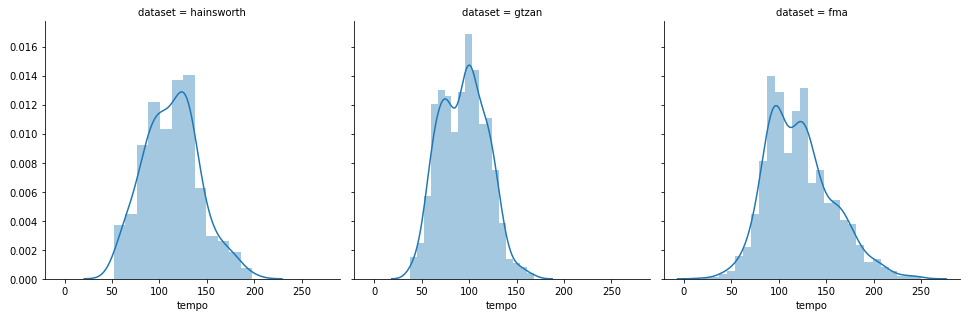
\includegraphics[width=0.9\textwidth]{Figures/distribucion_tempo_datasets.png}
  \caption{\textcolor{black}{Distribución de tempos en los sets de datos encontrados}.}
  \label{Fig:distribucion_tempo_datasets}
\end{figure}

Por otro lado, los géneros venían con distintos nombres o sub-etiquetas asociadas. Para simplificar el problema se han agrupado géneros similares y se han igualado nombres en todos los sets. Igualmente, el número de etiquetas no es el mismo en todos los sets, lo que hace tarea difícil unificarlos. Al comparar las distribuciones de géneros de cada fuente (Fig. \ref{Fig:distribucion_genero_datasets_1}), se ha comprobado que aún unificando etiquetas la calidad de éstas es muy distinta para cada set de datos.

\begin{figure}[htb]
  \centering
  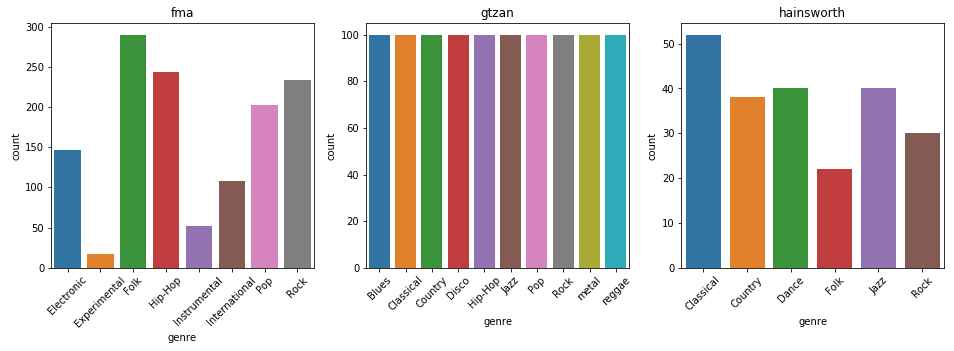
\includegraphics[width=0.9\textwidth]{Figures/distribucion_genero_datasets_1.png}
  \caption{\textcolor{black}{Distribución de género en los sets de datos encontrados}.}
  \label{Fig:distribucion_genero_datasets_1}
\end{figure}

Teniendo en cuenta número de casos y calidad de etiquetas se ha llegado a la conclusión de que el mejor set de datos es el set GTZAN y se utilizará éste exclusivamente en la investigación de la red y obtención de resultados.

\subsection{Procesamiento de datos de entrada}\label{sec:pre_process}
\noindent Dado que vamos a utilizar convoluciones 2D en nuestra red debemos convertir nuestros audios a matrices (imágenes) de dos dimensiones. Como ya se ha comentado en la revisión literaria, el proceso más común es la conversión de audio a espectrograma; para esto utilizaremos la librería \texttt{librosa} de Python. Además, para igualar todas las entradas a la red se van a tomar cortes de 3 segundos de los audios (con un solape del $50\%$ entre ellos para no perder información en el corte). 

\begin{figure}[htb]
  \centering
  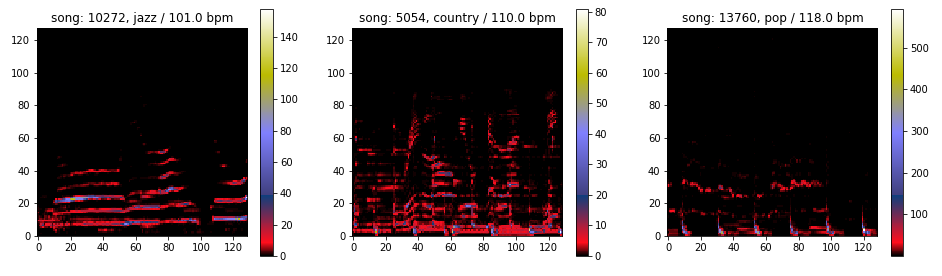
\includegraphics[width=0.9\textwidth]{Figures/espectrogramas2.png}
  \caption{\textcolor{black}{Espectrogramas de frecuencia}.}
  \label{Fig:espectrogramas}
\end{figure}

Los resultados de la conversión a espectrograma de los audios se puede ver en la Figura \ref{Fig:espectrogramas}. Aquí se muestran las frecuencias en el eje y, el tiempo del clip en el eje x y la densidad de la frecuencia en el eje z (representado con una escala de color). El uso de espectrogramas de éste modo es suficiente para entrenar la red, pero la representación de los datos en este momento es muy dispersa. Una forma de evitar esto es realizando una transformación de los datos usando las medias y desviaciones medias, pero como estamos tratando audios vamos a recurrir a una transformación logarítmica y representar los datos en decibelios (Figura \ref{Fig:espectrogramas_db}). 

\begin{figure}[htb]
  \centering
  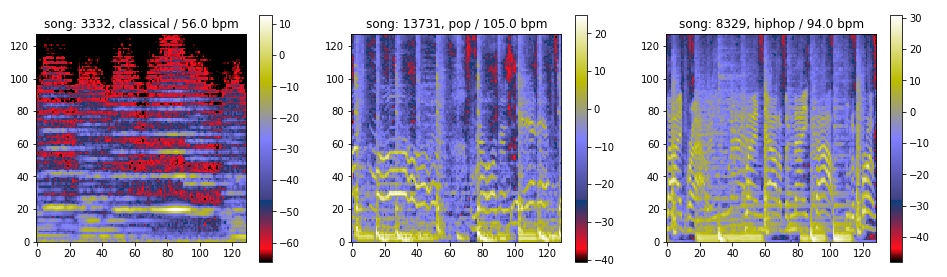
\includegraphics[width=0.9\textwidth]{Figures/espectrogramas_db2.png}
  \caption{\textcolor{black}{Espectrogramas de frecuencia en escala dB}.}
  \label{Fig:espectrogramas_db}
\end{figure}

Como se puede ver en la Figura \ref{Fig:espectrogramas_db} las imágenes ahora parecen contener más información en todas las áreas de la imagen y, además, una representación en decibelios es más afín a lo que el oído humano interpreta y por lo tanto a como se han grabado estos audios. Se espera que esto ayude a los modelos de predicción, aunque se harán pruebas con los dos tipos de datos para validar ésto.

\subsection{Procesamiento de datos de salida}\label{sec:target_process}

\noindent En las arquitecturas que se van a proponer se van a predecir dos variables distintas y éstas requieren su trato individual. 

El género se ha tratado como una variable cualitativa la cual tiene 10 clases, por lo que la variable se codificará en formato disperso o \textit{one-hot}. Los índices del vector que se han asignado a cada género se pueden ver en la Tabla \ref{tab:genre_classes}.

\begin{table}
\centering
\begin{tabular}{rllrl}
\hline
\textbf{Género} & \textbf{clase} &  & \textbf{Género} & \textbf{clase} \\ \hline
Metal			&	0			& 	&	Country			& 5  \\ 
Disco			&	1			& 	&	Pop			  & 6  \\ 
Clásica      	&	2			& 	&	Blues			& 7  \\ 
Hip-hop			&	3			& 	&	Reggae			& 8  \\ 
Jazz 			&	4			& 	&	Rock			& 9  \\ \hline
\end{tabular}
\caption{\textcolor{black}{Asignación de clases de géneros}}
\label{tab:genre_classes}
\end{table}

La variable tempo ha sido tratada de distintas maneras. Inicialmente se trató como una variable continua y se intentó predecir utilizando una activación lineal en la capa de salida pero esto no daba resultados muy prometedores. Como ya se ha visto en la Figura \ref{Fig:distribucion_tempo_datasets}, los datos siguen una distribución normal y por este motivo no se esperaba una mejora haciendo una normalización de los datos. Sin embargo al aplicar una transformación de este estilo se consigue que la variable tenga valores más cercanos a 0 (o 1) y un rango menor. Por este motivo, se intentó hacer normalizaciones sobre el tempo (\textit{min-max} y  estándar), pero, finalmente, no se consiguió que mejoraran los resultados.

Llegado este punto se re-estimó el problema y se planteó la variable de tempo como una variable discreta o cualitativa, por lo que se separaron los tempos en clases categóricas. En concreto, se construyeron dos variables de tempo. En la primera variable de tempo se creó una clase por valor de tempo en el set de datos (un total de 131 clases). La segunda variable y la que acabó dando resultados prometedores, divide el tempo en grupos de 10 como se muestra en la Tabla \ref{tab:tempo_classes}.

\begin{table}
\centering
\begin{tabular}{rllrl}
\hline
\textbf{Tempos} & \textbf{clase} &  & \textbf{Tempos} & \textbf{clase} \\ \hline
[38, 48]		&	0			& 	&	(108, 118]			& 7  \\ 
(48, 58]		&	1			& 	&	(118, 128]	  & 8  \\ 
(58, 68]		&	2			& 	&	(128, 138]		& 9  \\ 
(68, 78]		&	3			& 	&	(138, 148]		& 10  \\ 
(78, 88]		&	4			& 	&	(148, 158]		& 11  \\
(88, 98]		&	5			& 	&	(158, 168]		& 12  \\
(98, 108]		&	6			& 	&				&   \\  \hline
\end{tabular}
\caption{\textcolor{black}{Asignación de clases sobre la variable de tempo agrupado}}
\label{tab:tempo_classes}
\end{table}


\subsection{Partición de los datos}\label{sec:particion_de_datos}

\noindent La separación de los datos en los sets de entrenamiento y test se realizó utilizando la clase  \texttt{train\_test\_split} del paquete \texttt{scikit-learn} de Python. Se configuró una partición del $80\%$ de entrenamiento y un $20\%$ de test, apuntando a una distribución plana de las variables a predecir. Durante el entrenamiento se utilizó un $25\%$ de los datos de entrenamiento como set de validación, por lo que la partición total de entrenamiento, validación y test es del $60\%$, $20\%$, y $20\%$ de los datos totales respectivamente. Las dimensiones totales se pueden ver en la Tabla \ref{tab:variable_dim}.

\begin{table}[ht]
\centering
\begin{tabular}{llll}
\hline
\textbf{Variable} & \textbf{Entrenamiento} & \textbf{Validación} & \textbf{Test} \\ \hline
X (entrada) 		&	(11400, 128, 129, 1)				& 	(3800, 128, 129, 1)		& (3800, 128, 129, 1)  \\ 
género		&	(11400, 10)	&	(3800, 10)	  & (3800, 10)  \\ 
tempo		&	(11400, 1)	&	(3800, 1)	  & (3800, 1)   \\ 
tempo discreto		&	(11400, 131)	&	(3800, 131)	  & (3800, 131) \\ 
tempo agrupado		&	(11400, 13)	&	(3800, 13)	  & (3800, 13) \\ \hline
\end{tabular}
\caption{\textcolor{black}{Dimensiones de los datos utilizados para el entrenamiento de la red}}
\label{tab:variable_dim}
\end{table}

En la Figura \ref{Fig:distribucion_y} se puede ver la distribución de las variables objetivo con el corte entrenamiento/test. En la primera gráfica (de izquierda a derecha) se ve la variable de género, que está divida a partes iguales en todas las clases. Las dos gráficas restantes pertenecen a cortes sobre la variable de tempo agrupado. La gráfica de en medio muestra el número total de registros en cada clase de tempo y la gráfica de la derecha muestra las distribuciones de densidad de cada parte del corte. Ésta última hace que sea más visible que los cortes son de proporciones iguales en todas las clases.

\begin{figure}[htb]
  \centering
  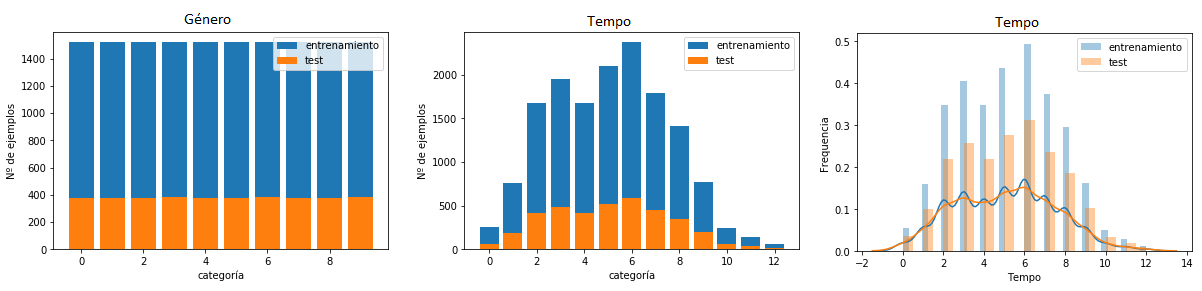
\includegraphics[width=\textwidth]{Figures/distribucion_y.png}
  \caption{\textcolor{black}{Distribución de las variables objetivo después del corte de entrenamiento y test}.}
  \label{Fig:distribucion_y}
\end{figure}


\section{Modelos y arquitecturas}\label{sec:arquitecturas}
\noindent El objetivo de este proyecto es diseñar una red que sea capaz de predecir género y tempo simultáneamente, para esto se debe de crear una red que tenga por lo menos dos ramas en la salida. Revisando la literatura se aprecia que los filtros verticales y horizontales procesados de forma separada y luego unidos mejoran la eficiencia de la extracción de información musical. Por lo que la red debería tener ramas paralelas interiormente además de la ramificación de salida (para las predicciones). Dada la complejidad del problema, se decidió diseñar la red por fases:
\begin{enumerate}
\item Diseño de una red CNN para predicción de género simple
\item Diseño de una red CNN para predicción de género con ramas paralelas de filtros verticales y horizontales
\item Diseño de una red CNN para la predicción de tempo
\item Diseño de una red CNN Para la predicción simultanea de género y tempo
\end{enumerate}

Varias arquitecturas se probaron en cada fase y fueron modificadas según las pruebas eran efectivas o no, a continuación se describen las arquitecturas principales probadas.

\subsection{Diseño de una red CNN simple para predicción de genero}\label{sec:arquitectura_simple}
\noindent La red que se utiliza aquí sirve como base para todas las demás, ésta es la arquitectura basada en el código de \cite{hguimares:gtzankeras}. La red simple de predicción de género tiene la siguiente estructura:
\begin{itemize}
\item \textbf{Entrada:} Imágenes de tamaño 128x129x1 (solo un canal)
\item \textbf{Bloque 1:}
\begin{itemize}
\item Convolución 2D: 16 filtros 3x3, activación relu
\item Pooling 2D: Maxpooling 2x2
\item Dropout: dropout del 25\% de activaciones
\end{itemize} 
\item \textbf{Bloque 2:}
\begin{itemize}
\item Convolución 2D: 32 filtros 3x3, activación relu
\item Pooling 2D: Maxpooling 2x2
\item Dropout: dropout del 25\% de activaciones
\end{itemize} 
\item \textbf{Bloque 3:}
\begin{itemize}
\item Convolución 2D: 64 filtros 3x3, activación relu
\item Pooling 2D: Maxpooling 2x2
\item Dropout: dropout del 25\% de activaciones
\end{itemize} 
\item \textbf{Bloque 4:}
\begin{itemize}
\item Convolución 2D: 128 filtros 3x3, activación relu
\item Pooling 2D: Maxpooling 2x2
\item Dropout: dropout del 25\% de activaciones
\end{itemize} 
\item \textbf{Bloque 5:}
\begin{itemize}
\item Convolución 2D: 64 filtros 3x3, activación relu
\item Pooling 2D: Maxpooling 4x4
\item Dropout: dropout del 25\% de activaciones
\end{itemize} 
\item \textbf{Salida:} Capa densa con 10 neuronas (salidas), activación softmax (para multi-clasificación)
\end{itemize}
        
Esta red funciona satisfactoriamente bien, como se vera en la sección de resultados, y por esto se ha dejado como está. Las siguientes arquitecturas son las que han necesitado un poco más de uso de la intuición además de refinamiento por prueba y error, pero todas utilizan bloques similares en cada convolución de Convolución 2D $\rightarrow$ Pooling (máx.) $\rightarrow$ Dropout (25\%).

\subsection{Diseño de una red CNN con ramas paralelas para predicción de genero}\label{sec:arquitectura_paralela}
\noindent En esta arquitectura se divide la red en dos ramas con filtros de estructura horizontal o vertical como se muestra en la Figura \ref{Fig:parallel_architecture}.

\begin{figure}[htb]
  \centering
  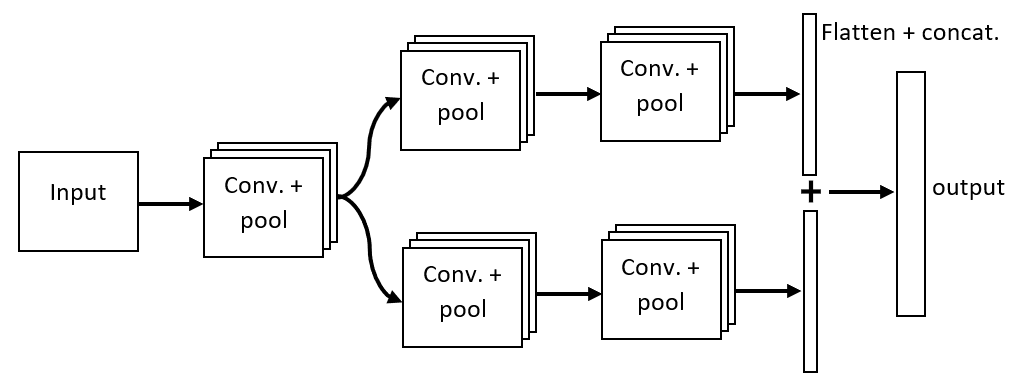
\includegraphics[width=\textwidth]{Figures/parallel_architecture.png}
  \caption{\textcolor{black}{Esquema de arquitectura de una red CNN con ramas paralelas}.}
  \label{Fig:parallel_architecture}
\end{figure}

La red tiene las mismas entradas y salidas que la red simple, al igual que el primer bloque de filtros convolucionales, pooling y dropout situado justo después de la entrada (sección \ref{sec:arquitectura_simple}). Los bloques de las dos ramas paralelas son como se describen a continuación:
\begin{itemize}
\item \textbf{Rama 1:} Filtros verticales
\begin{itemize}
\item \textbf{Bloque 1:}
\begin{itemize}
\item Convolución 2D: 32 filtros 8x2, activación relu
\item Pooling 2D: Maxpooling 2x2
\item Dropout: dropout del 25\% de activaciones
\end{itemize} 
\item \textbf{Bloque 2}
\begin{itemize}
\item Convolución 2D: 64 filtros 8x2, activación relu
\item Pooling 2D: Maxpooling 4x4
\item Dropout: dropout del 25\% de activaciones
\end{itemize} 
\end{itemize}
\item \textbf{Rama 2:} Filtros horizontales
\begin{itemize}
\item \textbf{Bloque 1:}
\begin{itemize}
\item Convolución 2D: 32 filtros 2x8, activación relu
\item Pooling 2D: Maxpooling 2x2
\item Dropout: dropout del 25\% de activaciones
\end{itemize} 
\item \textbf{Bloque 2:}
\begin{itemize}
\item Convolución 2D: 64 filtros 2x8, activación relu
\item Pooling 2D: Maxpooling 4x4
\item Dropout: dropout del 25\% de activaciones
\end{itemize} 
\end{itemize}
\end{itemize}

\subsection{Diseño de una red CNN para predicción de tempo}\label{sec:arquitectura_tempo}
\noindent Para el diseño de la red de predicción de tempo hubieron más iteraciones que para el resto. Inicialmente se hicieron pruebas con una red muy parecida a la red simple y con dos tipos de salidas: una salida de predicción numérica y otra de clasificación (Figura \ref{Fig:simple_tempo_architecture}).

\begin{figure}[htb]
  \centering
  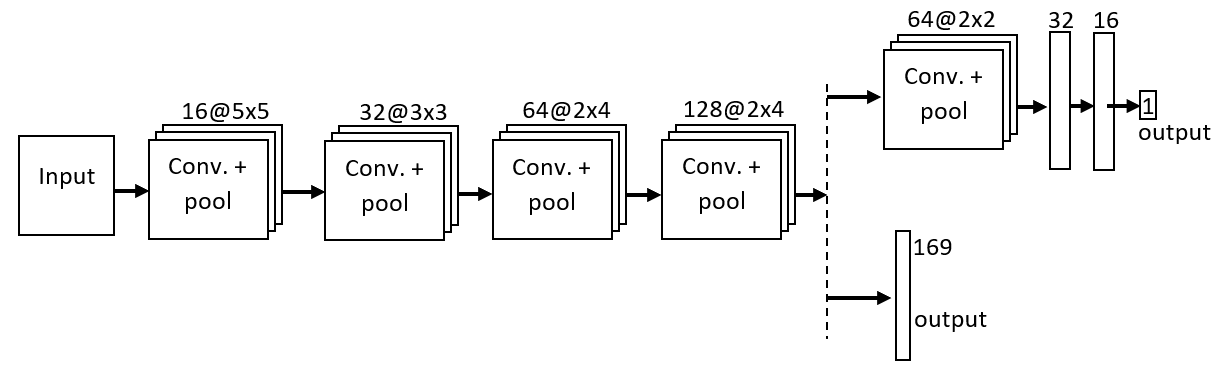
\includegraphics[width=\textwidth]{Figures/simple_tempo_architecture.png}
  \caption{\textcolor{black}{Esquema de arquitectura de una red CNN simple para predicción de tempo}.}
  \label{Fig:simple_tempo_architecture}
\end{figure}

En la Figura \ref{Fig:simple_tempo_architecture} se ve las dos arquitecturas iniciales para la predicción de tempo. Al igual que en las arquitecturas anteriores todos los bloques contienen Maxpooling y dropout. La arquitectura de la parte superior pertenece a la predicción numérica de tempo, con varias capas densas al final. La arquitectura de la parte inferior de la imagen pertenece a una predicción por clases, dónde cada clase era un número entero de tempo entre 38 y 168. Estas arquitecturas resultaron ser muy poco eficientes y se recurrió a filtros verticales y horizontales más alargados, acercándose ligeramente a los filtros vistos en la literatura.

La siguiente tanda de arquitecturas para tempo se componía de estructuras similares a la mostrada en la Figura \ref{Fig:simple_tempo_architecture}, pero con filtros horizontales y verticales de tamaño 8x2 y 2x7. La mayor estabilidad se obtuvo con una red de tres bloques de 8x2 (de 16, 32 y 32 filtros) seguida de dos bloques 2x7 (64 y 128 filtros) antes de los trozos finales para los dos tipos de red (numérica y clasificación). Aún siendo más estable y obteniendo menos sobreajuste, los resultados eran menos que satisfactorios. Llegados a este punto se decidió substituir la variable objetivo por el tempo agrupado (Tabla \ref{tab:tempo_classes}, sección \ref{sec:target_process}).

\begin{figure}[htb]
  \centering
  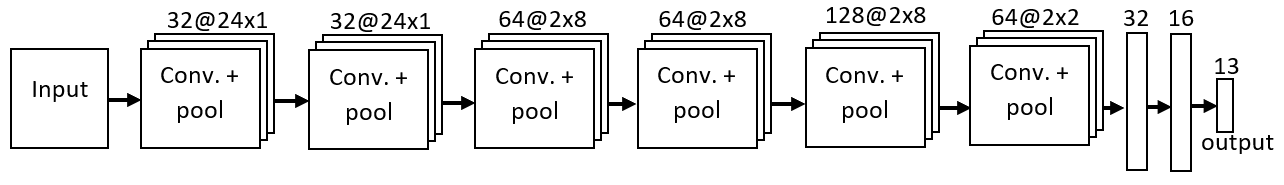
\includegraphics[width=\textwidth]{Figures/tempo_2_architecture.png}
  \caption{\textcolor{black}{Esquema de arquitectura de una red CNN para predicción de tempo agrupado con filtros verticales y horizontales (versión H2V)}.}
  \label{Fig:tempo_2_architecture}
\end{figure}

La figura \ref{Fig:tempo_2_architecture} muestra una red de tempo con filtros horizontales y verticales más definidos. Se hicieron dos variedades de esta red: la primera con los filtros mostrados en el esquema (versión H2V) y la segunda (versión V2H) con las dimensiones de los filtros intercambiadas, poniendo primero filtros horizontales seguidos de filtros vérticales (1x24 y 8x2 respectivamente). Estas dos redes llegaban rápido a una precisión mejor que las anteriores pero se estancaban. No obstante, se pensó que al juntar los predictores de género y tempo en una misma red la retro-propagación proveniente del género ayudaría a encontrar mejores filtros generales, al ser más estable.

\subsection{Diseño de una red CNN para predicción de género y tempo}\label{sec:arquitectura_mixed}

\noindent Al igual que con los problemas individuales se han probado dos arquitecturas distintas para éste problema. Inicialmente se probó con una arquitectura derivada de la red simple utilizando filtros genéricos de 3x3. Como ya se ha comentado en la sección anterior, aunque el tempo todavía no obtenga buenos resultados, se espera que la red aprenda mejor gracias a la estabilidad de la predicción de género.

\begin{figure}[htb]
  \centering
  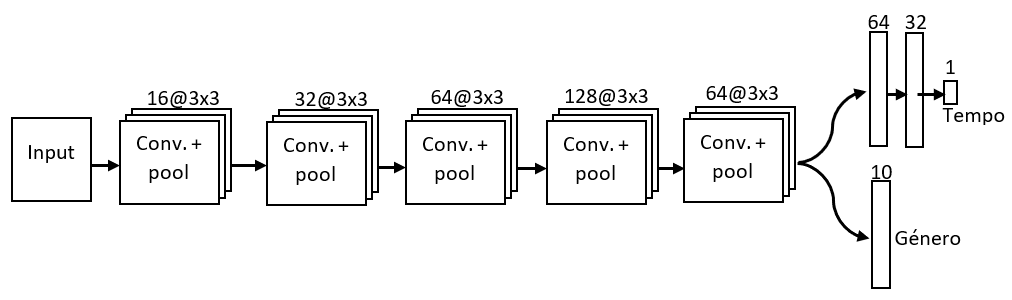
\includegraphics[width=\textwidth]{Figures/arquitectura_simple_mix.png}
  \caption{\textcolor{black}{Esquema de arquitectura de una red CNN simple para predicción de tempo y género}.}
  \label{Fig:arquitectura_simple_mix}
\end{figure}

La Figura \ref{Fig:arquitectura_simple_mix} muestra la estructura de la red que hace una predicción numérica del tempo y una clasificación de género. Nuevamente, al igual que todas las arquitecturas presentadas, cada bloque contiene una capa de Maxpooling y Dropout después de la convolución.

Finalmente, se juntaron todas las pruebas realizadas hasta el momento para hacer una propuesta de una red más estable capaz de predecir género y tempo. Para esta red se utilizó la variable de tempo agrupado teniendo dos clasificadores como salida de la red.

\begin{figure}[htb]
  \centering
  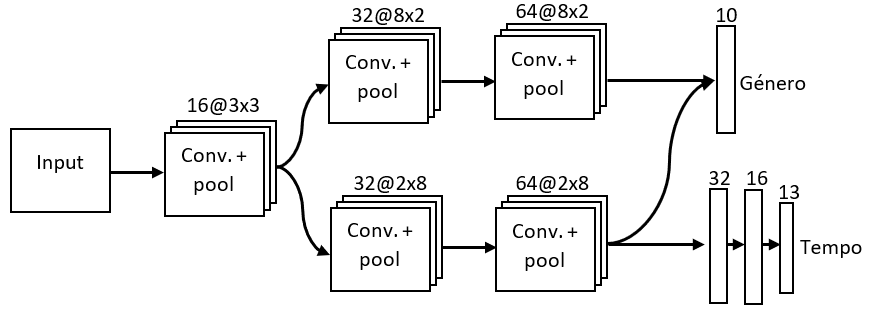
\includegraphics[width=\textwidth]{Figures/arquitectura_mix.png}
  \caption{\textcolor{black}{Esquema de arquitectura de una red CNN simple para predicción de tempo y género}.}
  \label{Fig:arquitectura_mix}
\end{figure}

La Figura \ref{Fig:arquitectura_mix} muestra una red con ramas paralelas de filtros horizontales y verticales que se unen para predecir la clase de género. Para el tempo es más importante sacar resolución temporal de intensidades que resolución sobre las frecuencias y por esto está solo conectado a la rama horizontal. Por otro lado el género es dependiente de las dos ramas y, al compartir rama con la predicción de tempo, se prevé que la retro-propagación del género ayude a aprender al tempo sin resultar perjudicados significativamente los pesos para predicción de género.

\subsection{Algoritmos de aprendizaje y otros meta-parámetros}\label{sec:metaparametros}
\noindent El énfasis de este estudio ha sido la arquitectura de la red, por lo que los meta-parámetros no arquitectónicos de la red no han sido explorados exhaustivamente. 

Para el algoritmo optimizador se han explorado los algoritmos RMSprop y ADAM con varios valores de ratio de aprendizaje inicial entre 0.1 y 0.001. Dado que el valor por defecto de 0.001 en ambos métodos daba la mayor estabilidad del algoritmo se ha elegido éste para todas las arquitecturas. Para predicción de género ADAM funcionaba bien, pero para predicción de tempo la utilización de RMSprop obtiene mejores estimaciones iniciales y ofreciendo estabilidad al modelo. Se piensa que la inclusión de momento con ADAM creaba modelos que se salían de la zona de aprendizaje cuando se trataba de predecir tempo.

Para el problema actual, especialmente con la entrada en decibelios, los valores positivos/grandes son más importantes que los negativos/pequeños, por este motivo se realiza \textit{maxpooling} después de las convoluciones siempre y se ha elegido la función de activación ReLU (Rectified Linear Unit). Para las predicciones multi-clase siempre se ha elegido una activación \textit{softmax}, mientras que las predicciones de valores de tempo se han hecho utilizando una activación lineal en la última capa.

La función de perdida utilizada para las clasificaciones es la de Entropía cruzada (\texttt{categorical\_crossentropy}) con una métrica de precisión (\texttt{accuracy}) para clases en las predicciones cualitativas y el error medio cuadrado para las predicciones numéricas, con una métrica del R$^2$. 

El valor del Dropout inicialmente estaba en torno al 25\%, pero debido a divergencias entre los valores de entrenamiento y validación, se amplió el ratio de Dropout al 50\% en varios modelos. 

Finalmente, se ha utilizado el valor de coste en los datos de validación para evaluar los modelos, al igual que para implementar un \textit{Early Stopping} y frenar el aprendizaje antes de que ocurra un sobre-ajuste o el modelo deje de aprender.

Los métodos importados para la construcción de las redes son del paquete Keras (utilizando el \textit{backend} de TensorFlow). Se ha utilizado el modo funcional de Keras para un mayor control de la arquitectura de la red y para la monitorización de los resultados se ha utilizado el paquete \texttt{tensorboard} de TensorFlow.

\section{Resultados}\label{sec:resultados}

\noindent En los siguientes apartados se van a comentar los resultados de las arquitecturas investigadas en la sección anterior. Para cada arquitectura se hicieron cambios de meta-parámetros hasta obtener resultados concluyentes utilizando los resultados de validación como objetivo.

Ninguno de los resultados obtenidos investigando la utilización del tempo como una variable continua fueron concluyentes y no entran en la discusión de resultados. No se encontró una arquitectura capaz de predecir esta variable resultando siempre en gradientes desvanecedoras y todas las predicciones de tempo al rededor de la media de la variable.

A continuación se presentará una discusión de los mejores resultados obtenidos en cada apartado, comparando las precisiones obtenidas en los datos de entrenamiento y test. Los resultados de entrenamiento de cada una de las redes discutidas se pueden ver en el apéndice \ref{Chapter:apendice_resultados}.

\subsection{Predicción de género}\label{sec:resultados_genero}

\noindent Como ya se ha comentado en apartados anteriores el género ha resultado ser una variable muy estable de predecir, siempre tiende a una solución con una precisión bastante alta. Por lo que ha resultado fácil hacer pruebas con ésta variable. Es posible que este resultado se deba a que cada género tiene una textura característica en representaciones por espectograma, lo que lo hace fácil de clasificar para una CNN. 

Una de las primeras pruebas que se realiza es la comparación de resultados cambiando la entrada entre un espectrograma directo o un espectrograma escalado en decibelios (Figuras \ref{Fig:espectrogramas} y \ref{Fig:espectrogramas_db} respectivamente).

\begin{table}[h]
%\centering
%\begin{tabular}{ccc}
%\textbf{}              & \textbf{Espectrograma simple} & \textbf{Espectrograma en dB} \\ \hline
%\textbf{Entrenamiento} & 0.90                          & 0.88                         \\
%\textbf{Test}          & 0.84                          & 0.83                         \\ \hline
\centering
\begin{tabular}{ccc}
\textbf{}                     & \textbf{Entrenamiento} & \textbf{Test} \\ \hline
\textbf{Espectrograma simple} & 0.90                   & 0.84          \\
\textbf{Espectrograma en dB}  & 0.88                   & 0.83          \\ \hline
\end{tabular}
\caption{\textcolor{black}{Precisión de la red de Género simple con respecto al formato de entrada}}
\label{tab:precision_genero_inputs}
\end{table}

En la Tabla \ref{tab:precision_genero_inputs} se muestra la comparación de precisiones para la red simple de predicción de género cambiando la entrada. Al contrario de lo que se pensaba al diseñar la red, la red distingue mejor el género en la imagen no tratada que en la imagen transformada a decibelios. Esto se debe a que al estandarizar las imágenes la red tiene más dificultades para distinguir imágenes parecidas, ya que todas ellas acaban con un aspecto (textura) similar.

Similarmente, se compara la arquitectura paralela (Figura \ref{Fig:parallel_architecture}) con la arquitectura simple para predicción de género. Como muestra la Tabla \ref{tab:precision_genero_paralelo} Los resultados son ligeramente inferiores para la arquitectura paralela. Ésto es de esperar ya que en redes profundas la serielización es más potente que la paralelización. A pesar de esto, la red de arquitectura paralela sigue teniendo una precisión buena.

\begin{table}[h]
\centering
\begin{tabular}{ccc}
\textbf{}                     & \textbf{Entrenamiento} & \textbf{Test} \\ \hline
\textbf{Red simple} & 0.90                   & 0.84          \\
\textbf{Red paralela}  & 0.88                   & 0.82          \\ \hline
\end{tabular}
\caption{\textcolor{black}{Comparación de precisión de las redes de Género simple y paralela.}}
\label{tab:precision_genero_paralelo}
\end{table}

\subsection{Predicción de tempo}\label{sec:resultados_tempo}

\noindent La red de predicción de tempo fue más complicada de construir para que tuviera resultados aceptables. La mayoría de arquitecturas daban precisiones (o valores de R$^2$ en el caso de las predicciones numéricas) muy malas o dejaban de aprender rápidamente topándose con gradientes desvanecedoras. Finalmente se hicieron dos variedades una red CNN muy profunda (mostrada en la Figura \ref{Fig:tempo_2_architecture}). La primera variedad tiene filtros 24x1 seguidos de filtros 2x8 (que llamaremos V2H) y en la segunda variedad se invierten las dimensiones con filtros de 1x24 seguidos de filtros 8x2 (que llamaremos H2V). En ambas redes se predice el tempo agrupado en 13 clases. Estas redes siguen teniendo un aprendizaje poco estable, pero llegan rápidamente a una solución aceptable.

\begin{table}[h]
\centering
\begin{tabular}{ccc}
\textbf{}                 & \textbf{Entrenamiento} & \textbf{Test} \\ \hline
\textbf{Red H2V} & 0.57                   & 0.57          \\
\textbf{Red V2H} & 0.56                   & 0.50          \\ \hline
\end{tabular}
\caption{\textcolor{black}{Comparación de precisión de las redes de predicción de tempo.}}
\label{tab:precision_tempo}
\end{table}

En la Tabla \ref{tab:precision_tempo} se comparan las precisiones de estas dos últimas redes de predicción de tempo. Las dos tienen una precisión similar en entrenamiento con una gran diferencia: la red con filtros verticales seguidos de horizontales (V2H) presenta sobre-ajuste mientras que la otra no tiene ningún sobre-ajuste. Comparando los resultados con la literatura se llega a la conclusión de que, como los filtros verticales son más importantes para la predicción de tempo, el uso de filtros horizontales después de los verticales impide el entrenamiento de éstos. Debido a estos resultados se elige utilizar filtros principalmente verticales para la predicción de tempo en la red conjunta.

\subsection{Predicción de género y tempo}\label{sec:resultados_mix}

\noindent Para la predicción de género y tempo se realizaron dos pruebas principales. La primera prueba se realizó con una arquitectura simple (Figura \ref{Fig:arquitectura_simple_mix}). Esta prueba se realizó antes de conseguir ningún resultado satisfactorio con la red de tempo y el objetivo era comprobar que, al juntar género y tempo, los pesos aprendidos para la variable de género ayudarían a predecir el tempo. El resultado muestra que el tempo mejora gracias al género como se esperaba, pero al mismo tiempo la precisión del género disminuía considerablemente (Tabla \ref{tab:precision_mix_simple}). 

\begin{table}[htb]
\centering
\begin{tabular}{ccc}
\textbf{}       & \textbf{Entrenamiento} & \textbf{Test} \\ \hline
\textbf{Género} & 0.35                   & 0.41          \\
\textbf{Tempo (R$^2$)}  & 0.03                   & 0.004         \\ \hline
\end{tabular}
\caption{\textcolor{black}{Precisión (R$^2$ en este caso de Tempo) de la red simple con predicciones de género y tempo.}}
\label{tab:precision_mix_simple}
\end{table}

Finalmente, utilizando todo lo aprendido en las pruebas anteriores, se diseñó y probó una red con ramas paralelas (Fig. \ref{Fig:arquitectura_mix}) que predice género y tempo de manera satisfactoria. En esta red el género de nuevo pierde precisión a favor de una mejora en la precisión del tempo, pero esta vez ambas variables obtienen buenos resultados de precisión como puede observarse en la Tabla \ref{tab:precision_mix_paralela}.

\begin{table}[htb]
\centering
\begin{tabular}{ccc}
\textbf{}       & \textbf{Entrenamiento} & \textbf{Test} \\ \hline
\textbf{Género} & 0.82                   & 0.78          \\
\textbf{Tempo}  & 0.68                   & 0.62         \\ \hline
\end{tabular}
\caption{\textcolor{black}{Precisión de la red final con predicciones de género y tempo.}}
\label{tab:precision_mix_paralela}
\end{table}

A modo de cerrar el círculo de pruebas, se repitió el entrenamiento de la red final utilizando los espectrogramas escalados a decibelios para ver si los resultados obtenidos con la red simple de género se replican con el modelo final. 

\begin{table}[htb]
\centering
\begin{tabular}{ccc}
\textbf{}       & \textbf{Entrenamiento} & \textbf{Test} \\ \hline
\textbf{Género} & 0.77                   & 0.66          \\
\textbf{Tempo}  & 0.67                   & 0.65         \\ \hline
\end{tabular}
\caption{\textcolor{black}{Precisión de la red final con predicciones de género y tempo utilizando espectrogramas escalados a decibelios.}}
\label{tab:precision_mix_paralela_db}
\end{table}

Comparando las Tablas \ref{tab:precision_mix_paralela} y \ref{tab:precision_mix_paralela_db}, se puede observar que la precisión del género sigue empeorando cuando se usan espectrogramas en decibelios. Sin embargo, los espectrogramas en decibelios parecen ayudar a la precisión del tempo. Se sospecha que la conversión a decibelios resalta los pulsos en un rango más amplio del espectrograma, lo que los hace más distinguibles para la predicción de tempo.

\section{Conclusión}\label{sec:conclusion}

\noindent En este trabajo se ha investigado el estado de los algoritmos y modelos de extracción de información musical (MIR) en el campo del aprendizaje profundo. Así mismo, se han investigado parámetros y arquitecturas CNN para su uso en la predicción de características rítmicas de audios de música. Las características elegidas han sido género y tempo, dada su importancia para determinar el ritmo de una pieza musical.

Las investigaciones sobre género han demostrado que las CNN son excepcionales para la clasificación de ésta variable. Estos modelos son más efectivos cuando se utilizan espectrogramas no escalados ni estandarizados, aunque un escalado en decibelios no daña significativamente la precisión.

Las investigaciones sobre tempo han demostrado que, en efecto, la selección de filtros principalmente verticales o horizontales es muy importante de cara a la eficiencia del modelo. Por lo tanto se debe tener cuidado al elegir el orden de filtros horizontales y verticales. Por otro lado, la predicción de tempo se ha visto mejorada por la utilización de espectrogramas escalados con decibelios. Este fenómeno está causado por la ampliación de intensidades de pulso sobre todas las frecuencias al convertir el espectrograma a decibelios.

Finalmente, se ha demostrado que se puede construir un modelo que prediga simultáneamente género y tempo. En un modelo conjunto la variable más estable y fácilmente predecible por la red (el género) ha ayudado a entrenar los pesos para predecir una variable mucho más complicada (el tempo).

Estos resultados no son totalmente concluyentes, ya que todavía se pueden incluir mejoras al modelo introduciendo más capas en cada rama o continuando la investigación del efecto de la alteración de los espectrogramas sobre la precisión. También, se podría investigar el uso de otras activaciones o algoritmos de aprendizaje alternativos al ADAM o el RMSprop.

En conclusión, este estudio sugiere que la predicción de ritmos en la música es posible, ya que un modelo bastante modesto ha sido capaz de predecir género y tempo de un set de datos de sólo 8 horas de música.